En fælles samarbejdsaftale blev lavet \cref{fig:SAftale}, med aftaler om mødetider og regler omkring brugen af software og værktøjer \cref{fig:4}. Aftalen blev lavet i en skriftlig udgave, fordi så kunne man nemmere referer til arket hvis der kom tvivl om hvad der var aftalt. Samt at alle i gruppen kunne skrive under for at vise at de gik med i hvad der var nedskrevet.

\begin{figure}[ht!]
  \centering
  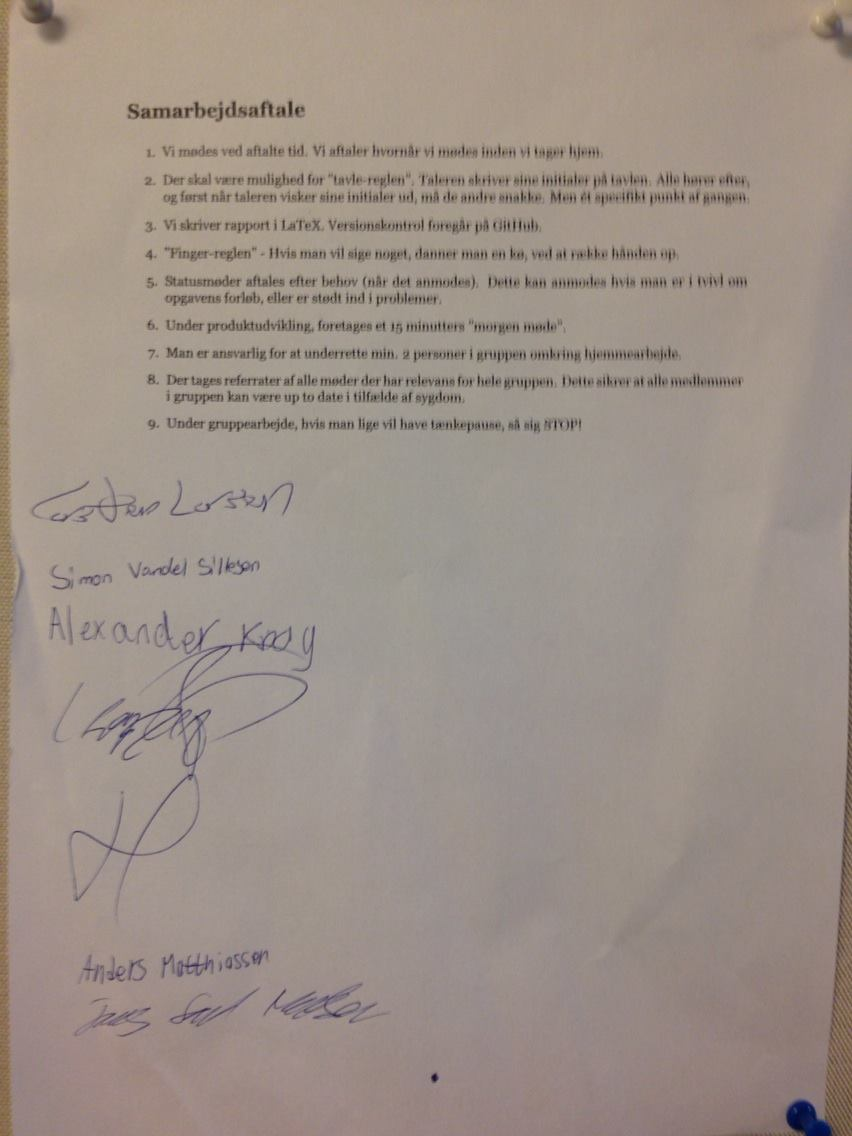
\includegraphics[width=0.5\textwidth]{Images/S_Aftale.jpg}
  \caption{nada}
  \label{fig:SAftale}
\end{figure}

\begin{figure}[ht!]
    \centering
    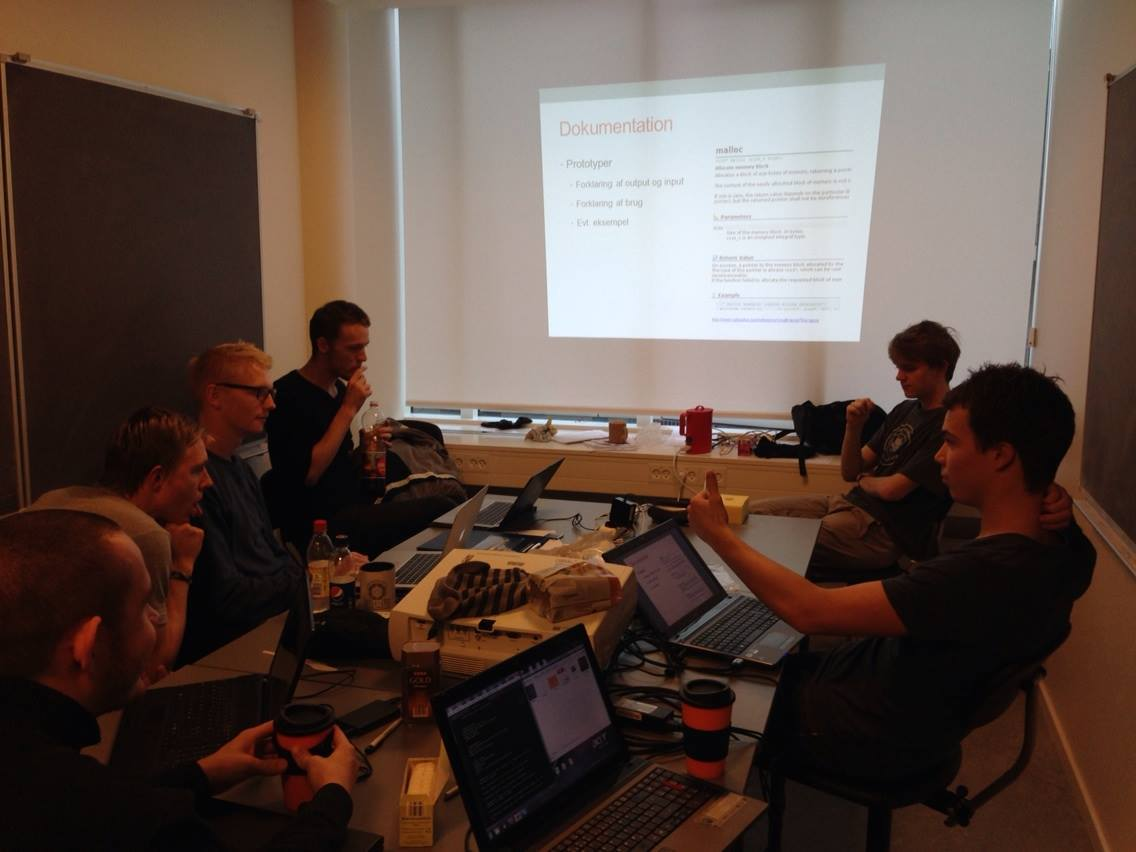
\includegraphics[width=0.5\textwidth]{Images/8.jpg}
    \caption{BAH}
    \label{fig:4}
\end{figure}
Gruppen har været enige om et ambitionsniveau, i forhold til hvad der ar forventet af projektet og kvaliteten af arbejdet. Udenfor projektarbejdet har der været en generel deltagelse i sociale aktiviteter, fordi at det har været godt for at danne sociale relationer til andre grupper, og for at styrke sammenholdet indbyrdes i gruppen. Der blev dog kun deltaget i arrangementer når at projektet var godt med i forhold til tidsplanen. 
Der har som regel været møde med hovedvejleder hver uge, og bivejleder på samme måde, dog med en nedskæring da projektet nærmede sig sin slutning. De opfølgende møder blev aftalt til sidst af hvert møde. Under de daglige møder har der også været en plan, hvis det var at nogle medlemmer ikke mødte op. Hvis et eller flere gruppemedlemmer ikke var mødt op til aftalt tid, og der heller ikke var givet besked, ville gruppemedlemmet blive ringet op af et andet medlem. Hvis opkaldet ikke blev besvaret ville en besked blive vedlagt, og efter en given tidsperiode (et kvarters tids) ville der blive lavet endnu et et opkald i så fald at der ikke var kommunikeret noget tilbage endnu. Når alle var til stede og vores møder begyndte var det velset at man deltog i diskussionerne og at man kom med input. Hvis nogen gruppemedlemmer var meget stille, ville de andre ind spørge til personens mening om det der var emnet for diskussionen. Når der har været en diskussion som har været meget omfattende og gruppemedlemmerne begyndte at afbryde hinanden, blev der taget et "finger system" i brug. Det gik ud på at hvis et gruppemedlem havde noget de ville have sagt i diskussionen, skulle man række en finger i vejret. Den næste der ville sige noget skulle så vise to fingre og den tredje tre finger og så videre. Når den første fik ordet ville han tage fingeren ned og de andre i køen vil vise en finger mindre. På den måde ville der altid kun være en som havde ordet af gangen, og derved blev der ikke brugt for meget tid på at diskutere.

To femte dele inde i projektet da størstedelen af fokussen lå i at skrive analyse var motivationen ikke så høj. Det var grundet i at analysedelen ikke var noget som gruppen fandt videre interessant, dog giv arbejdsmoral op igen da projektet blev mere løsningsorienteret. Under hele projektet blev arbejdsopgaverne fordelt efter interesse og der var aldrig én som alene havde ansvar for en opgave. Det betød at der var mulighed for at delegere en person en opgave, men stadig have flere til at tage ansvar for at opgaven blev lavet.
Gruppen har primært arbejdet i mindre inddelte grupper, fordi at hvis mange tildeles en opgave bliver den ikke nødvendigvis bedre resultater. Også fordi gruppen regelmæssig diskuterede, har det været godt at lave grupperne så en diskussion ikke har stoppet alt arbejdet, men at den gruppe som arbejdede med opgaven kunne tage diskussionen og derved komme frem til afgørelse. Vi har sammensat gruppen efter Belbins team-rolle model, for at gruppen skal kunne begå sig i en bred sammenhæng af situationer. Når der har skulle udeles kritik, blev en begrundelse givet mundtligt og skriftlig i form af noter eller samtaler. Kritikken blev altid modtaget med en begrundelse for hvorfor noget skulle ændres.

\section{Vurdering - Hvordan gik det}
\paragraph{Samarbejdsaftale}
Finger reglen som var nedskrevet blev taget i brug indtil at gruppen var blevet bedre til ikke at afbryde hinanden og give mere plads. Gruppen var også gode til skrive referater under hvert vejlederemøde, hvilket var en opgave som folk selv meldte sig til. I starten af projektet var gruppen god til at aftale hvornår det var at næste møde skulle finde sted, i forhold til mødetid og hvornår man regnede med at tage hjem igen. Forsinkelser blev indberettet hvis man var forsinket, disse meddelelser kom indenfor 20 minutter, når man var sikker på at det ikke var muligt at møde op til den aftalte mødetid. Dog senere hen i projektet blev det mere sløvt med at melde sig forsinket hvis man ikke kunne komme til den aftalte tid.

\paragraph{Gruppetrivselen}
Gruppen har været god til at sørge for at der er en god stemning i lokalet og når der har været et arrangement. Ofte efter at dagens arbejde var over, har der været tid til et spil kort eller en film. Når der har været frokostpause, har gruppen sendt to mand ned for at hente brød og pålæg, for at kunne have fællesspisning i grupperummet bagefter. Alle betalte så deres andel af udgifterne ligegyldigt hvor meget man spiste eller ikke spiste. Dog har der været problemer med at ingen rydde op efter maden.

\paragraph{Lektier og arbejdsopgaver}
Der manglede ofte overblik over hvad der var lavet og hvad folk arbejde på. Det har så betydet at hvis nogen har skrevet i det samme dokument har man skulle bruge tid på flette teksterne sammen, hvilket har været spild af tid. Når der var udeligeret lektier til næste dag, var det heller ikke at alting blev lavet. Enten fordi at man ikke kunne finde tid til dem eller fordi man havde gabt over mere end man kunne sluge. Når man ville komme med kritik af et stykke arbejde har gruppen ikke været for nådefulde og derved ikke kommet med alt kritikken. 

\section{Analyse - Hvorfor gik det som det gik}
Grundet stædighed har der opstået problem med mange og lange diskussion, hvilket har resulteret i at vores projekt har kørt så glidende som det kunne have gjort. Der blev fortaget kompromisser, når der skulle tages beslutninger som et tilfælde endte med en halvfærdig løsning.
På grund at af gruppe blev bedre til at diskutere, efter at have praktiseret finger reglen, blev gruppemedlemmerne også bedre til at vente med at tale for en anden var færdig. Det har betydet at diskussionerne har været mere flydende.

Fordi at gruppen har brugt meget tid på at spille kort og lave andre hyggelige eller sjove aktiviteter, har det betydet at når der skulle arbejdes igen har det været med en god morale. Pauserne har også været fælles så der ikke er nogen som er blevet forstyrret under arbejdet. 

\section{Syntese}
\paragraph{Dette vil vi begynde at gøre i P2, som vi ikke gjorde i P1}
Der skal være en som tager ansvarsrollen som ham der skal holde styr på hvad der foregår i en uge af gangen. Han skal have styr på hvad der skal laves, hvad der er lavet, hvad der bliver lavet og hvem der gør hvad. Han skal også sørge for at folk bliver færdig med de opgaver som de fik tildelt.


\paragraph{Dette vil vi ikke gøre i P2, som vi gjorde i P1}
Vi vil stoppe med et efterlade madrester, bestik og andre fødevarer i grupperummet, da det efterladte både en dårlig lugt og velkomst til dem som mødte op først. 

\paragraph{Dette vil vi fortsætte med at gøre (gerne anderledes og bedre) i P2, som vi også gjorde i P1}
Vi vil fortsætte med at deltage i sociale arrangementer og aktiviteter efter arbejde. 